\documentclass[12pt,a4paper]{report}

\usepackage{bookman}
\usepackage{ngerman}
\usepackage[T1]{fontenc}
\usepackage[utf8]{inputenc}
\usepackage{graphicx}
\usepackage[left=2cm,right=2cm,top=2cm,bottom=2cm]{geometry}

\begin{document}

	\Huge Theodor Fontane
	\hspace{2cm}
	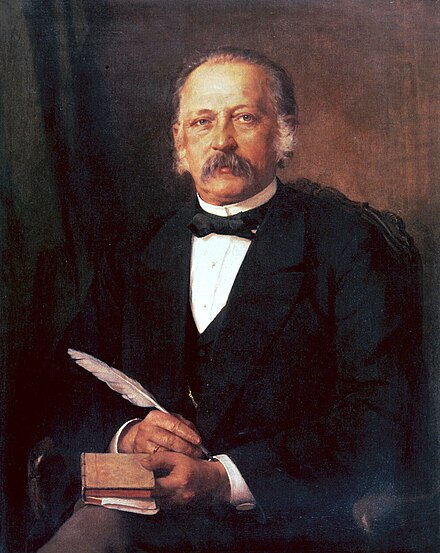
\includegraphics[width=4cm]{IMG_1135.jpeg}

	\vspace{1cm}
	\normalsize
	
	\paragraph{Generelles}
	
	\begin{itemize}
		\item Geboren wurde er am 30. Dezember 1819 in Neuruppin
		\item Gestorben ist er am 20. September 1898 in Berlin
	\end{itemize}
	
	\paragraph{Familie}
	
	\begin{itemize}
		\item Er hatte sieben Kinder, eine Schwester
		\item Seine Mutter (Emilie Fontane) hieß genauso, wie seine Ehefrau
		\item Sein Vater hieß Louis Henry Fontane
	\end{itemize}
	
	\paragraph{Leben}
	
	\begin{itemize}
		\item Arbeitete als Apothekergehilfe
		\item Von 1. April 1844 bis zum 31 März 1845 leistete er freiwilligen Millitädienst.
		\item Veröffentlichte 1839 seine erste Novelle \dq Geschwisterliebe\dq
		\item Er arbeitete als Journalist
		\item Ab 1849 gab er den Apothekerberuf völlig auf, um als freier Schriftsteller zu leben.
	\end{itemize}
	
	\paragraph{Bedeutung und Stil}
	
	\begin{itemize}
		\item Vertreter des poetischen Realismus
		\item All seine Werke sind aus einem auktorialen Gestus (auktorialer Erzähler) erzählt (manchmal Abweichung zum personalen Erzähler)
	\end{itemize}

	
\end{document}